% Options for packages loaded elsewhere
\PassOptionsToPackage{unicode}{hyperref}
\PassOptionsToPackage{hyphens}{url}
%
\documentclass[
]{article}
\usepackage{lmodern}
\usepackage{amssymb,amsmath}
\usepackage{ifxetex,ifluatex}
\ifnum 0\ifxetex 1\fi\ifluatex 1\fi=0 % if pdftex
  \usepackage[T1]{fontenc}
  \usepackage[utf8]{inputenc}
  \usepackage{textcomp} % provide euro and other symbols
\else % if luatex or xetex
  \usepackage{unicode-math}
  \defaultfontfeatures{Scale=MatchLowercase}
  \defaultfontfeatures[\rmfamily]{Ligatures=TeX,Scale=1}
\fi
% Use upquote if available, for straight quotes in verbatim environments
\IfFileExists{upquote.sty}{\usepackage{upquote}}{}
\IfFileExists{microtype.sty}{% use microtype if available
  \usepackage[]{microtype}
  \UseMicrotypeSet[protrusion]{basicmath} % disable protrusion for tt fonts
}{}
\makeatletter
\@ifundefined{KOMAClassName}{% if non-KOMA class
  \IfFileExists{parskip.sty}{%
    \usepackage{parskip}
  }{% else
    \setlength{\parindent}{0pt}
    \setlength{\parskip}{6pt plus 2pt minus 1pt}}
}{% if KOMA class
  \KOMAoptions{parskip=half}}
\makeatother
\usepackage{xcolor}
\IfFileExists{xurl.sty}{\usepackage{xurl}}{} % add URL line breaks if available
\IfFileExists{bookmark.sty}{\usepackage{bookmark}}{\usepackage{hyperref}}
\hypersetup{
  pdftitle={Predictive Modeling Exercises},
  pdfauthor={Kessiena Ofunrein, Jordan Pflum, Jennifer Robinson, and Katelyn Vincent},
  hidelinks,
  pdfcreator={LaTeX via pandoc}}
\urlstyle{same} % disable monospaced font for URLs
\usepackage[margin=1in]{geometry}
\usepackage{graphicx,grffile}
\makeatletter
\def\maxwidth{\ifdim\Gin@nat@width>\linewidth\linewidth\else\Gin@nat@width\fi}
\def\maxheight{\ifdim\Gin@nat@height>\textheight\textheight\else\Gin@nat@height\fi}
\makeatother
% Scale images if necessary, so that they will not overflow the page
% margins by default, and it is still possible to overwrite the defaults
% using explicit options in \includegraphics[width, height, ...]{}
\setkeys{Gin}{width=\maxwidth,height=\maxheight,keepaspectratio}
% Set default figure placement to htbp
\makeatletter
\def\fps@figure{htbp}
\makeatother
\setlength{\emergencystretch}{3em} % prevent overfull lines
\providecommand{\tightlist}{%
  \setlength{\itemsep}{0pt}\setlength{\parskip}{0pt}}
\setcounter{secnumdepth}{-\maxdimen} % remove section numbering
\usepackage{placeins}
\usepackage{tikz}
\usetikzlibrary{mindmap,shadows}

\title{Predictive Modeling Exercises}
\author{Kessiena Ofunrein, Jordan Pflum, Jennifer Robinson, and Katelyn Vincent}
\date{8/8/2020}

\begin{document}
\maketitle

\hypertarget{question-1-done}{%
\section{Question 1 DONE}\label{question-1-done}}

Though potentially accurate in their findings, the conclusions of the
initial analysis regarding the economic viability of ``going green''
were based on flawed logic. The employee filtered out buildings with
occupancy rates of less than ten percent, assuming that the occupancy
rate for the new building will be over ten percent without providing
evidence to support his theory. To strengthen his argument, he could
have used a visual like the one below, which shows the leasing rates by
size for all of the buildings in the data set. Based on this, it appears
that there are in fact no `green' buildings in the data set with leasing
rates (aka occupancy rates) lower than 10 percent.

\begin{center}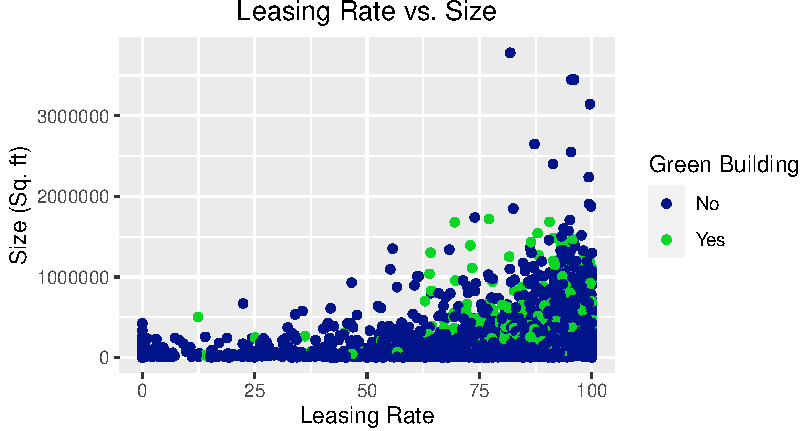
\includegraphics{STA380Exercises_Ofunrein_Pflum_Robinson_Vincent_files/figure-latex/unnamed-chunk-2-1} \end{center}

While the idea of filtering the dataset is a good one, the filtering
approach did not take into account the information that is known about
the new project - that it will be a 15-story mixed-use building in
Austin, TX measuring 250,000 sq. ft. This information, though limited,
allows us to narrow our focus to buildings with similar properties. For
example, we created a subset of the data that contained information
about buildings that: were between 10-20 stories, were either less than
10 years old or had been renovated, had amenities (since the building
will be mixed-use), and had annual cooling degree days over 966 (the
median for the whole dataset). Since there were no variables directly
related to location, we used high cooling degree days to filter on
locations in similar climates to Austin, TX (if not similar geographic
regions). This subset contained 407 buildings, including 33 designated
as `green buildings'.\\
Subsetting the data yields different information about the rent of green
vs non-green buildings. Below is the rent distribution for all buildings
in the dataset, which would seem to support the original analysis.

\begin{center}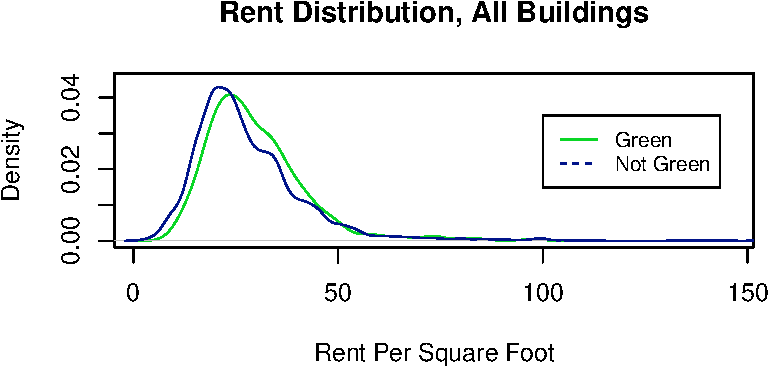
\includegraphics{STA380Exercises_Ofunrein_Pflum_Robinson_Vincent_files/figure-latex/unnamed-chunk-3-1} \end{center}

However, when analyzing green buildings in the subset of data
(containing information on buildings similar to the new one), it appears
that the rent distribution skews slightly more towards less expensive
rental prices.

\begin{center}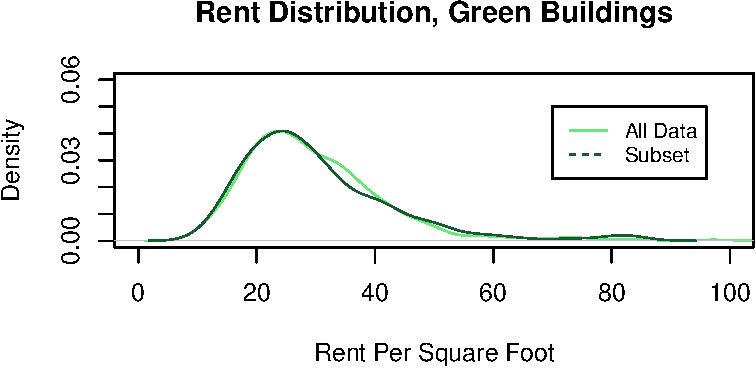
\includegraphics{STA380Exercises_Ofunrein_Pflum_Robinson_Vincent_files/figure-latex/unnamed-chunk-4-1} \end{center}

The median rent for green buildings in the subset is 24.36 dollars vs
22.50 dollars, this is still higher, but both are significantly less
than the rental prices in the original analysis.

\begin{center}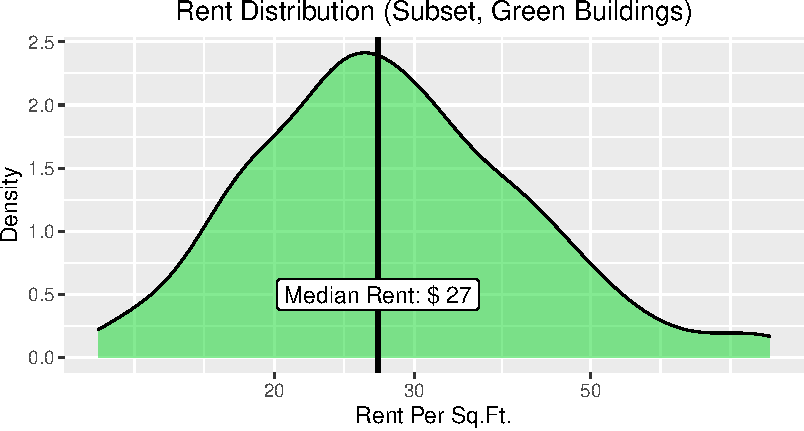
\includegraphics{STA380Exercises_Ofunrein_Pflum_Robinson_Vincent_files/figure-latex/unnamed-chunk-5-1} \end{center}

\begin{verbatim}
## The following objects are masked from df (pos = 3):
## 
##     age, amenities, cd_total_07, class_a, class_b, cluster,
##     cluster_rent, CS_PropertyID, Electricity_Costs, empl_gr,
##     Energystar, Gas_Costs, green_rating, hd_total07, leasing_rate,
##     LEED, net, Precipitation, renovated, Rent, size, stories,
##     total_dd_07
\end{verbatim}

\begin{center}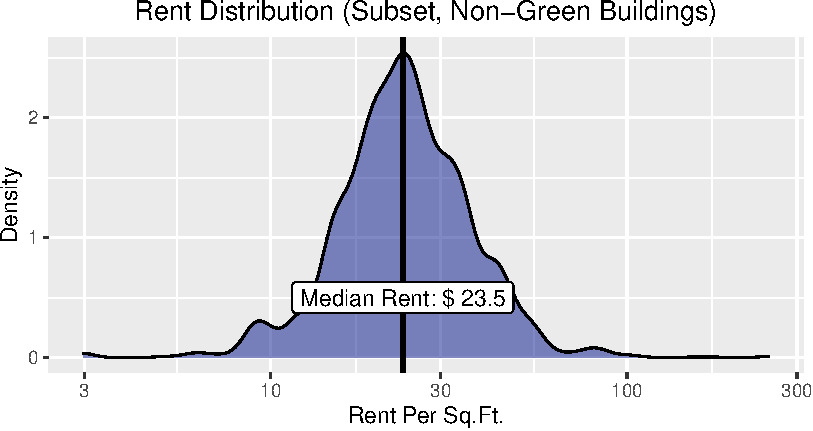
\includegraphics{STA380Exercises_Ofunrein_Pflum_Robinson_Vincent_files/figure-latex/unnamed-chunk-5-2} \end{center}

Additionally, while the original analysis factored in expected revenue
differences, it failed to account for differences in electricity cost
savings over the year from ``going green''. Only three percent of all
buildings (and six percent of green buildings) in the original dataset
have rent quoted on a ``net contract'' basis, where the tenant pays for
utility costs, which means that the majority of utility costs are paid
by the building owners.\\
Estimated annual electricity costs for a non-green building were
computed using the building size (250,000 sq ft), avg number of kWh per
square foot for commercial buildings (22.5), and median electricity
costs for buildings in the subset. The annual electricity costs for the
green building assumed a 25 percent reduction in energy usage. To
compute revenue, the median occupancy rate was multiplied by the median
rent (for green and non-green buildings in the subset, separately).
Below is the break-even analysis for a new green building, which takes
into account the difference in costs and expected revenues compared to
the construction of a non-green building. Based on this analysis, the
additional costs of the green building would be recouped in 9.5 years.

\begin{center}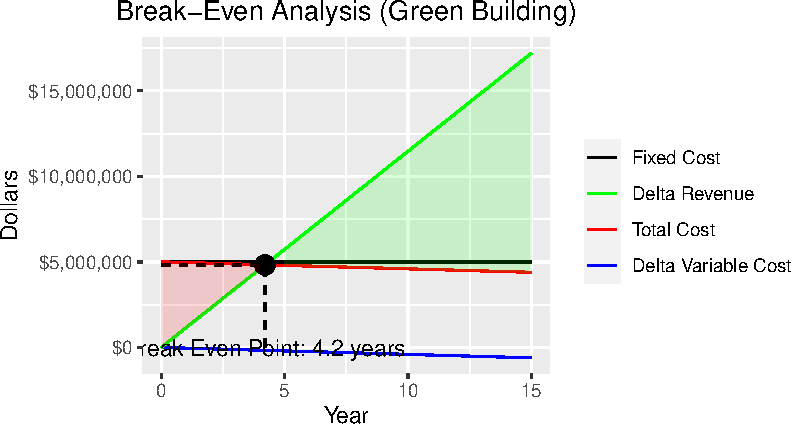
\includegraphics{STA380Exercises_Ofunrein_Pflum_Robinson_Vincent_files/figure-latex/unnamed-chunk-6-1} \end{center}

One possible confounding variable for the relationship between rent and
green status in the initial analysis could be the building class. Almost
80\% of all green buildings are Class A buildings, which are the highest
quality buildings in a market, whereas only 36 percent of non-green
buildings have a Class A designation. Since Class A buildings command a
much higher rent than other building types, what appeared to be a higher
rent for `green' buildings could be attributed to the fact that most of
them are of a higher quality building type.

\begin{verbatim}
## The following objects are masked from df (pos = 3):
## 
##     age, amenities, cd_total_07, class_a, class_b, cluster,
##     cluster_rent, CS_PropertyID, Electricity_Costs, empl_gr,
##     Energystar, Gas_Costs, green_rating, hd_total07, leasing_rate,
##     LEED, net, Precipitation, renovated, Rent, size, stories,
##     total_dd_07
\end{verbatim}

\begin{verbatim}
## The following objects are masked from df (pos = 4):
## 
##     age, amenities, cd_total_07, class_a, class_b, cluster,
##     cluster_rent, CS_PropertyID, Electricity_Costs, empl_gr,
##     Energystar, Gas_Costs, green_rating, hd_total07, leasing_rate,
##     LEED, net, Precipitation, renovated, Rent, size, stories,
##     total_dd_07
\end{verbatim}

\begin{center}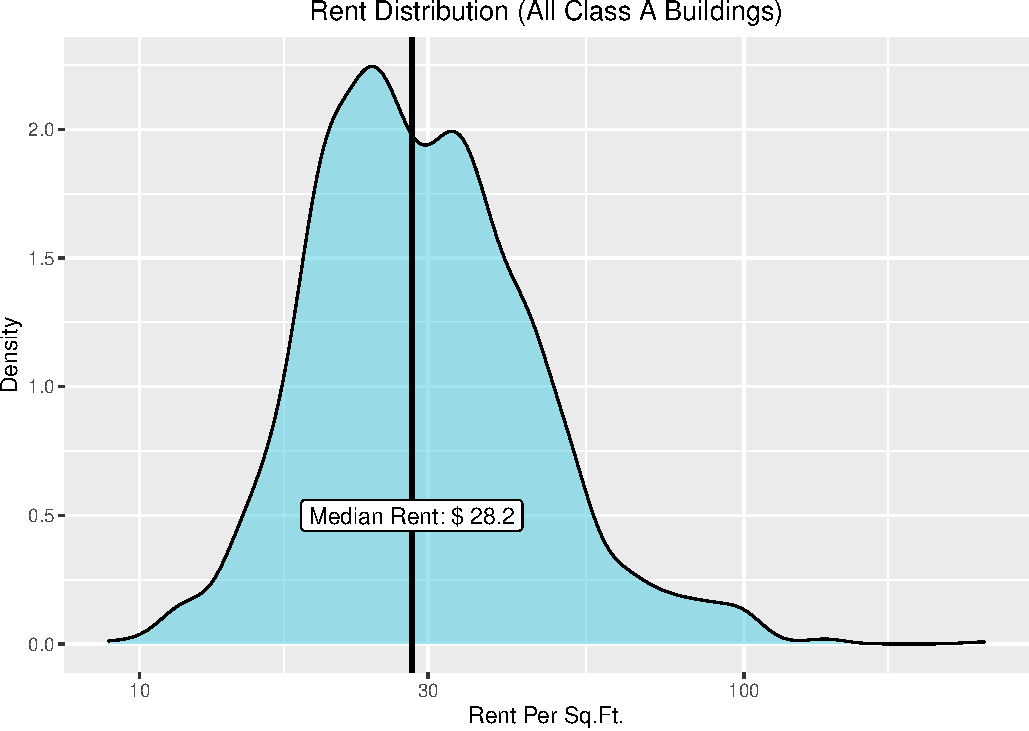
\includegraphics{STA380Exercises_Ofunrein_Pflum_Robinson_Vincent_files/figure-latex/unnamed-chunk-7-1} \end{center}

\begin{verbatim}
## The following objects are masked from df (pos = 3):
## 
##     age, amenities, cd_total_07, class_a, class_b, cluster,
##     cluster_rent, CS_PropertyID, Electricity_Costs, empl_gr,
##     Energystar, Gas_Costs, green_rating, hd_total07, leasing_rate,
##     LEED, net, Precipitation, renovated, Rent, size, stories,
##     total_dd_07
## 
## The following objects are masked from df (pos = 4):
## 
##     age, amenities, cd_total_07, class_a, class_b, cluster,
##     cluster_rent, CS_PropertyID, Electricity_Costs, empl_gr,
##     Energystar, Gas_Costs, green_rating, hd_total07, leasing_rate,
##     LEED, net, Precipitation, renovated, Rent, size, stories,
##     total_dd_07
\end{verbatim}

\begin{verbatim}
## The following objects are masked from df (pos = 5):
## 
##     age, amenities, cd_total_07, class_a, class_b, cluster,
##     cluster_rent, CS_PropertyID, Electricity_Costs, empl_gr,
##     Energystar, Gas_Costs, green_rating, hd_total07, leasing_rate,
##     LEED, net, Precipitation, renovated, Rent, size, stories,
##     total_dd_07
\end{verbatim}

\begin{center}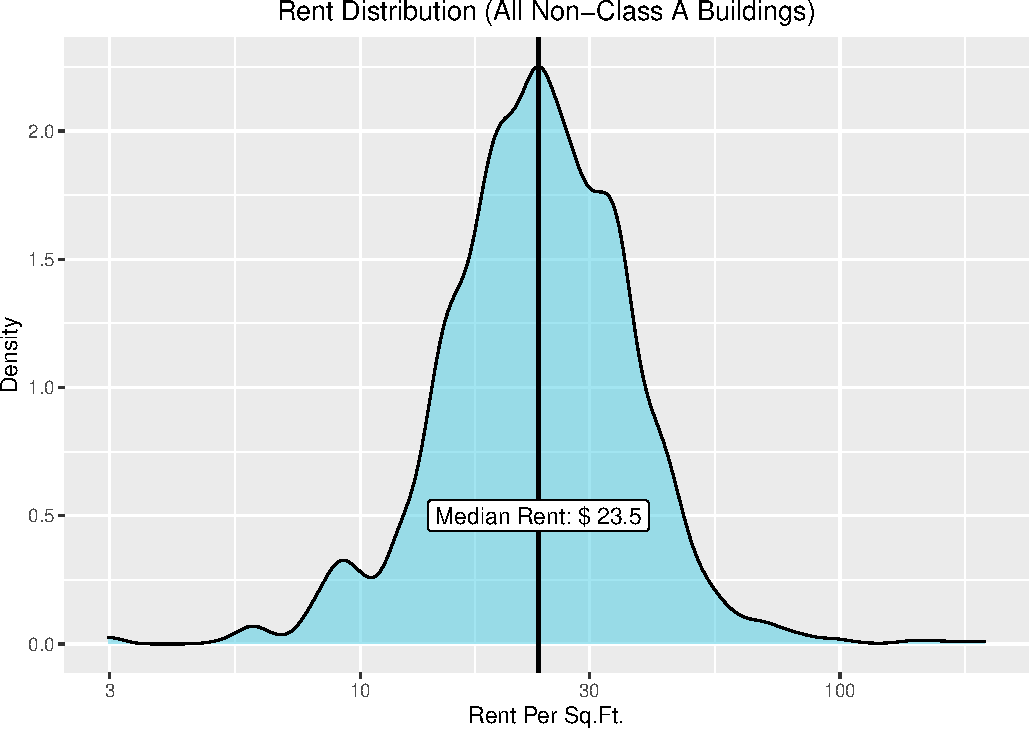
\includegraphics{STA380Exercises_Ofunrein_Pflum_Robinson_Vincent_files/figure-latex/unnamed-chunk-7-2} \end{center}

\hypertarget{question-2-done}{%
\section{Question 2 DONE}\label{question-2-done}}

The figures below portray a story about the flights arriving in and
departing from the Austin Bergstrom International Airport in 2008. We
looked at traits of flights and airlines from a few different
perspectives to convey an accurate image of what the airport and
travelers experienced that year. This analysis of the data is extremely
useful for a few different potential clients. Firstly, travelers are the
sustenance of this industry and are impacted by the factors we are
analyzing. By providing them with some of these graphs, travelers will
be more informed about some things they are likely to experience
temporally, geographically, or with a specific airline. Secondly,
airport officials would benefit greatly from our analysis because it is
advantageous to know what one is likely to experience with each airport.
Airports are businesses with reputations and standards. Notoriety for
delayed flights is very useful information for preparations and
strategic planning.

The line graph figures below are a time series analysis of how the
length of flight delays changes throughout the year 2018. The graphs are
relatively similar and have peaks during similar times. They are
separated by arriving and departing flights, essentially whether the
plane was late coming in or late coming out. It is to be expected that a
change in one would impact an airport's schedule thus resulting in
changes in the other. For both graphs there are peaks in months like
March, June, and December. It is easy to deduce the cause of that could
be holidays or related to school schedules like Spring Break. For a more
concrete picture further analysis should be conducted. The airlines
graphed here have more flights than the average airline and the delays
are considered long delays because they are in the 75th percentile.

\begin{verbatim}
## `summarise()` regrouping output by 'Month' (override with `.groups` argument)
\end{verbatim}

\begin{center}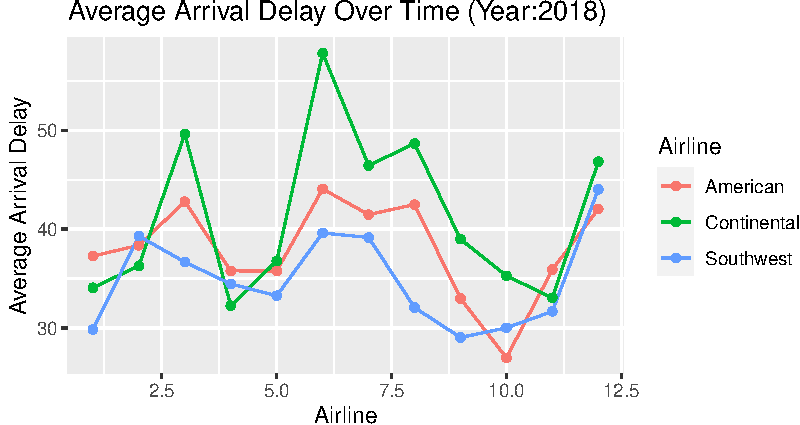
\includegraphics{STA380Exercises_Ofunrein_Pflum_Robinson_Vincent_files/figure-latex/unnamed-chunk-9-1} \end{center}

\begin{verbatim}
## `summarise()` regrouping output by 'Month' (override with `.groups` argument)
\end{verbatim}

\begin{center}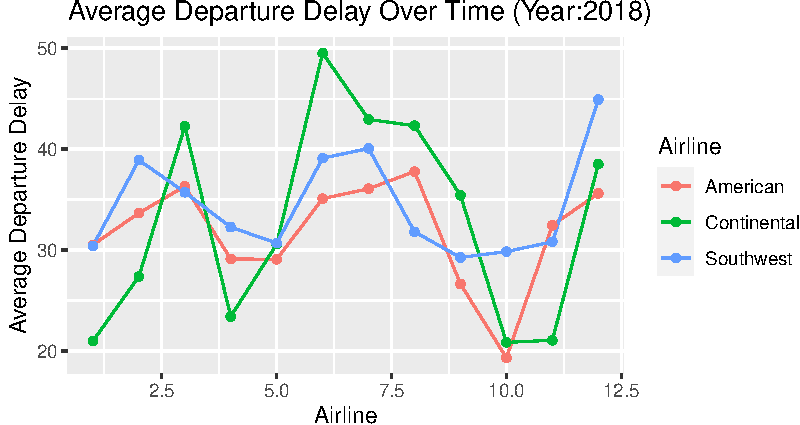
\includegraphics{STA380Exercises_Ofunrein_Pflum_Robinson_Vincent_files/figure-latex/unnamed-chunk-9-2} \end{center}

As we transition our focus from how flights are delayed for longer
periods of time seasonally, we can also look at the different types of
cancellations and delays. The graph below enables us to compare three
types of cancellation codes: Carrier, Weather, and NAS. This plot is
clearly able to show that NAS delays do not account for many delays and
truly do not compare to weather or carrier delays.

\begin{verbatim}
## `summarise()` regrouping output by 'CancellationCode' (override with `.groups` argument)
\end{verbatim}

\begin{center}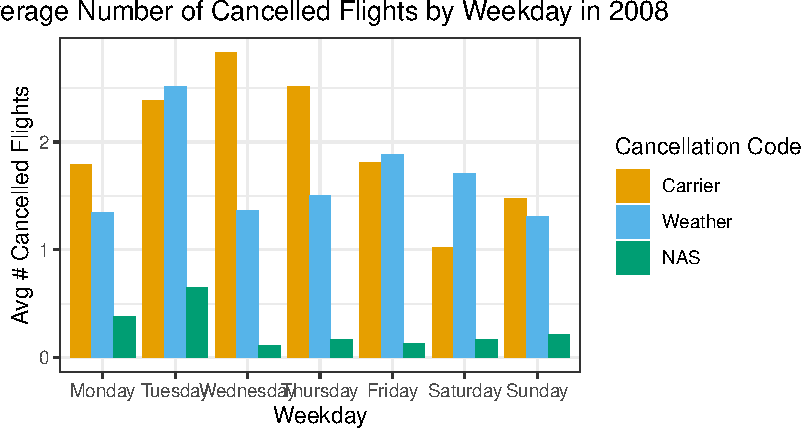
\includegraphics{STA380Exercises_Ofunrein_Pflum_Robinson_Vincent_files/figure-latex/unnamed-chunk-10-1} \end{center}

In the graph below, we look at a similar trend but over months so we can
look at a seasonal picture of the flights. Some interesting anomalies
are found in April and September. Based on knowledge of seasonal changes
in weather, one could conclude that the significant flux in weather
delays in September could be explained by hurricane season. As for
April, carrier delays could increased significantly because American
Airlines canceled a lot of flights due to not meeting government
regulation standards.

\begin{verbatim}
## `summarise()` regrouping output by 'CancellationCode' (override with `.groups` argument)
\end{verbatim}

\begin{center}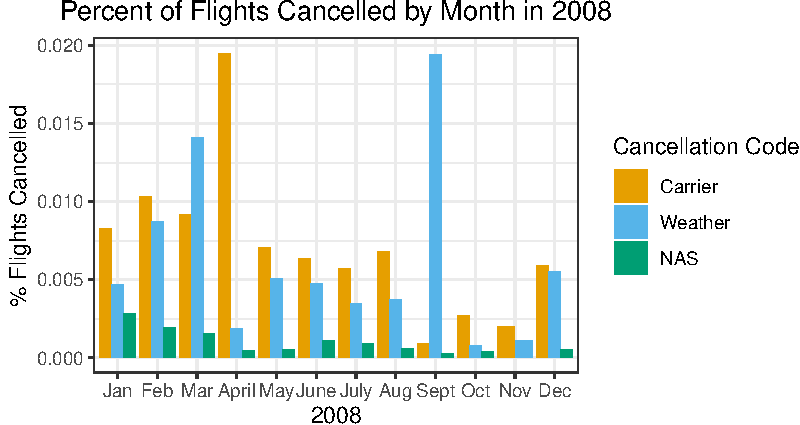
\includegraphics{STA380Exercises_Ofunrein_Pflum_Robinson_Vincent_files/figure-latex/unnamed-chunk-11-1} \end{center}

Strategic planning is a fundamental component of how airports sustain
themselves. Knowing that an airport or region is notorious for delays or
that they are notorious for this seasonally, plans can be made to
accommodate to yield the best options for travelers. A simple way to
summarize this information in a plot is through geographical mapping.
Figure \_\_\_ shows this; airports with larger volumes of flights
arriving in or departing from Austin have larger and brighter circles.
An airport official should show more concern for a large dot that is
lightly shaded, as this airport has a lot of flights outgoing to the
Austin airport so schedules in these airports are integral to an
efficient airport.

\begin{verbatim}
## Source : http://tile.stamen.com/toner-lite/4/2/5.png
\end{verbatim}

\begin{verbatim}
## Source : http://tile.stamen.com/toner-lite/4/3/5.png
\end{verbatim}

\begin{verbatim}
## Source : http://tile.stamen.com/toner-lite/4/4/5.png
\end{verbatim}

\begin{verbatim}
## Source : http://tile.stamen.com/toner-lite/4/5/5.png
\end{verbatim}

\begin{verbatim}
## Source : http://tile.stamen.com/toner-lite/4/2/6.png
\end{verbatim}

\begin{verbatim}
## Source : http://tile.stamen.com/toner-lite/4/3/6.png
\end{verbatim}

\begin{verbatim}
## Source : http://tile.stamen.com/toner-lite/4/4/6.png
\end{verbatim}

\begin{verbatim}
## Source : http://tile.stamen.com/toner-lite/4/5/6.png
\end{verbatim}

\begin{verbatim}
## `summarise()` ungrouping output (override with `.groups` argument)
\end{verbatim}

\begin{center}\includegraphics{STA380Exercises_Ofunrein_Pflum_Robinson_Vincent_files/figure-latex/unnamed-chunk-14-1} \end{center}

\begin{verbatim}
## `summarise()` ungrouping output (override with `.groups` argument)
\end{verbatim}

\begin{center}\includegraphics{STA380Exercises_Ofunrein_Pflum_Robinson_Vincent_files/figure-latex/unnamed-chunk-14-2} \end{center}

Now that we have an understanding of where the most frequented airports
are, we can now look at a similar map that tells us how timely these
airports' flights are. Similar to the most frequented locations, in the
graphs below we see the locations with the most airports still have
larger circles, but lighter colors represent longer delays on average
for the year. We know from previous graphs the length of delays is
somewhat seasonal, but on average we see that the more frequented
airports do not have relatively long delays. We actually notice in
states like Iowa there is not a lot of flights from here but they have a
significantly higher average length of delay. We see something similar
for flights arriving in Tennessee.

\begin{verbatim}
## `summarise()` ungrouping output (override with `.groups` argument)
\end{verbatim}

\begin{center}\includegraphics{STA380Exercises_Ofunrein_Pflum_Robinson_Vincent_files/figure-latex/unnamed-chunk-15-1} \end{center}

\begin{verbatim}
## `summarise()` ungrouping output (override with `.groups` argument)
\end{verbatim}

\begin{center}\includegraphics{STA380Exercises_Ofunrein_Pflum_Robinson_Vincent_files/figure-latex/unnamed-chunk-15-2} \end{center}

\hypertarget{question-3-done}{%
\section{Question 3 DONE}\label{question-3-done}}

Our group chose to construct a simple portfolio of three ETFs: iShares
Core U.S. Aggregate Bond ETF (AGG), SPDR Gold Shares (GLD), Vanguard
Growth Index Fund ETF Shares (VUG). We chose AGG because it is
considered a relatively safe investment and would help mitigate the
volatility of VUG. Additionally, we selected GLD, an ETF which tracks
the price of Gold (\textasciitilde1/10) as Gold has been a hot commodity
in the wake of COVID-19 and the expected rise in inflation rates. Figure
1 depicts the Cumulative Return, Daily Return, and Drawdown of each of
the assets.

\begin{center}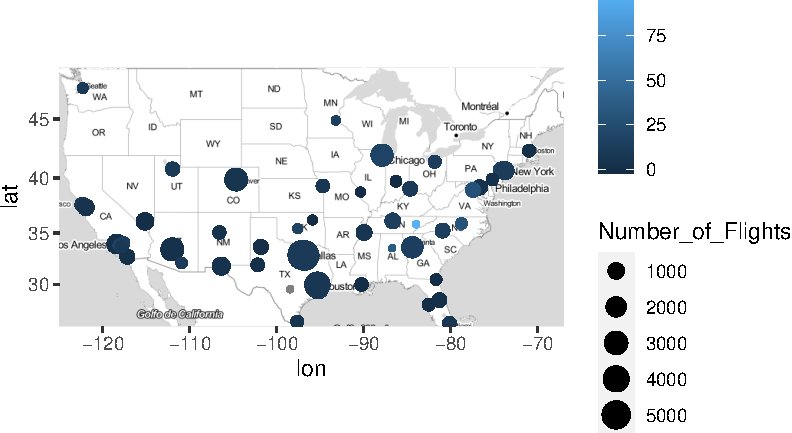
\includegraphics{STA380Exercises_Ofunrein_Pflum_Robinson_Vincent_files/figure-latex/unnamed-chunk-17-1} \end{center}

The top chart unsurprisingly shows that VUG has the highest cumulative
return over the past five years (as it is the most risky investment of
the three) and AGG as the lowest. However, it is also apparent that GLD
has high returns in the past 6 months and nears the cumulative return of
VUG. The bottom graph depicts the drawdown for every asset during each
period. The drawdown of an asset refers to how much an investment or
trading account is down from the peak before it recovers back to the
peak. Therefore, it is generally a good measure of the negative risk of
an asset.

\begin{center}\includegraphics{STA380Exercises_Ofunrein_Pflum_Robinson_Vincent_files/figure-latex/unnamed-chunk-18-1} \end{center}

Figure 1 does not do the best job of displaying the return of an asset
in respect to the risk taken on. Therefore, Figure 2 plots the
annualized return for every asset vs annualized risk (SD). You can see
that VUG has the highest risk of all three assets but the also the
highest return. One last graph that is useful to examine is each of the
assets relative performance to the market. To simplify things, we used
SPY, and ETF that track the S and P500, as our market proxy. Figure 3
shows each of the assets performance relative to SPY. If SPY were
graphed, it would be a horizontal line intersection the y-axis at 1.
Therefore, whenever an asset is above 1, they are performing better than
the market.

\begin{center}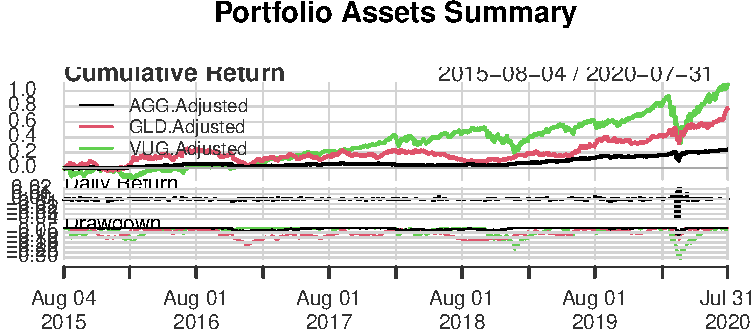
\includegraphics{STA380Exercises_Ofunrein_Pflum_Robinson_Vincent_files/figure-latex/unnamed-chunk-19-1} \end{center}

We can see that VUG has consistently been beating the market while the
less risky assets GLD and AGG have not, although GLD has made a recent
push above the market.

These three figures confirm our initial thoughts of the risk-reward
ratio of each of the assets and why we chose them to comprise our
portfolio. However, we then needed to decide how much to invest in each
of the assets in our portfolio.

We decided for our first portfolio, Portfolio 1, we would create a very
safe portfolio to satisfy a client who was risk-averse. Therefore, we
invested heavily in AGG (0.8), lightly in GLD (0.15) and almost nothing
in VUG (0.05).

For our second portfolio we decided to invest risky, perhaps for a young
client with a lot of new wealth and in the position to take on financial
risk. For this portfolio, Portfolio 2, we invested heavily in VUG (0.7),
moderately in GLD (0.2) and lightly in AGG (0.1).

Lastly, we constructed our third portfolio by optimizing our portfolio
(in respect to Variance) subject to a set of constraints: Full
Investment: \(\sum_{i} w_i =1, \forall\)portfolios No Over/Under
Investment: \(0.05 \leq w_i \leq0.05 \forall\)portfolios Target Return
(about 10 percent annual): \(w' \bar\mu = 0.00055\) Our objective was to
minimize the variance of the portfolio given the constraints listed
above. This resulted in a portfolio with: \(w_{AGG}\)=0.0659
\(w_{GLD}\)=0.500 \(w_{VUG}\)=0.4341 A summary of our portfolio weights
can be seen in Table 1.

\[\begin{table}[!h]
\begin{tabular}{llll}
Portfolio   & Weight (AGG) & Weight (GLD) & WeightVUG \\
Portfolio 1 & 0.8          & 0.15         & 0.05      \\
Portfolio 2 & 0.1          & 0.2          & 0.7       \\
Portfolio 3 & 0.0659       & 0.5          & 0.4341   
\end{tabular}
\end{table}\] The portfolios constructed above yielded the following
numbers (monthly) (Table2):

\[\begin{table}[!h]
\begin{tabular}{lllll}
Portfolio   & Return (Percent) & Risk (Percent) & Sharpe Ratio & VaR (Percent) \\
Portfolio 1 & 0.49             & 1.38           & 0.356        & -1.696        \\
Portfolio 2 & 1.78             & 4.05           & 0.70.289     & -5.55         \\
Portfolio 3 & 1.11             & 3.08           & 0.356        & -4.033       
\end{tabular}
\end{table}\]

The table does a nice job of summarizing the portfolios. Portfolio 1,
which is the safest of the three, has the lowest return and the lowest
VaR. However, although Portfolio 2 has a higher return than portfolio 3,
it has a much higher risk and VaR than Portfolio 3 and therefore a
considerably lower Sharpe Ratio. Because Portfolio 3 was optimized, it
had a much better relative performance than Portfolio 2.

\begin{center}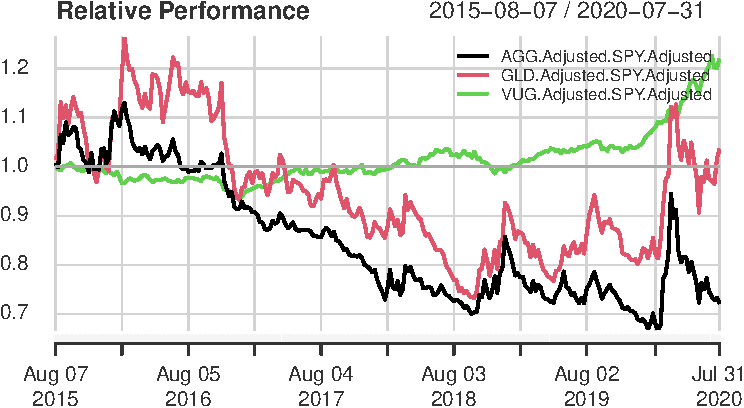
\includegraphics{STA380Exercises_Ofunrein_Pflum_Robinson_Vincent_files/figure-latex/unnamed-chunk-21-1} \end{center}

Figure 4 does a good job of illustrating the table information. With
little risk, Portfolio 1's distribution is skinny and high, indicating
narrow but consistent returns. However, although Portfolio 2's and 3's
returns are very similar, Portfolio 2's risk and VaR are a lot lower.
This can most noticeably be seen in the levels of VaR (plotted as dashed
vertical lines). The interpretation of the VaR line is simple:

VaR(95) = -4.033: Your portfolio has a 5 percent chance of losing 4.033
percent or more in a given month.

It is also useful to translate our portfolio to dollars. Let's assume
that we have 100,000 dollars to invest in our portfolio. Table 3 shows
the monthly Expected Return, Risk, and VaR of each portfolio. For
example, in any given month, our portfolio (3) would be expected to grow
on average 1,105 dollars. We would be 95 percent confident that it would
grow within the range of -5057 dollars and 7,267 dollars. Finally, we
would expect there to be a 5 percent chance that we would lose 4,022
dollars in any given month.

\[\begin{table}[!h]
\begin{tabular}{llll}
Portfolio   & Return (Dollars) & Risk (Dollars) & VaR (Dollars) \\
Portfolio 1 & 498              & 1384           & -1686         \\
Portfolio 2 & 1178             & 4045           & -5587         \\
Portfolio 3 & 1105             & 3081           & -4022        
\end{tabular}
\end{table}\] \# Question 4

\hypertarget{question-5}{%
\section{Question 5}\label{question-5}}

\hypertarget{question-6-done}{%
\section{Question 6 DONE}\label{question-6-done}}

Initial exploration of the grocery dataset reveals that the top three
most frequently purchased items are whole milk, other vegetables, and
rolls/buns. The top twenty most frequently purchased items are shown in
the figure below. The list includes common pantry and fridge staples you
would expect to see in most grocery carts, such as milk, dairy products,
fruit and vegetables, soda and beer, bread, juice, and eggs.

\begin{center}\includegraphics{STA380Exercises_Ofunrein_Pflum_Robinson_Vincent_files/figure-latex/unnamed-chunk-25-1} \end{center}

On the other end, the least frequently purchased items include a lot of
non-food items, including toiletries (hairspray, makeup remover),
cleaning and organization products (rubbing alcohol, toilet cleaner,
bags), and baby products (baby food and baby cosmetics).

\begin{center}\includegraphics{STA380Exercises_Ofunrein_Pflum_Robinson_Vincent_files/figure-latex/unnamed-chunk-26-1} \end{center}

Looking at the association rules with the highest support, we see that
some of the most popular items are also the items most frequently
purchased together, which makes sense. For example, whole milk and other
vegetables were purchased together in 7.5 percent percent of all
transactions, the highest of any pair of items. In fact, the majority of
rules with high support include whole milk or other vegetables. The
other two combinations of items included in at least 5percent of
shoppers' carts include whole milk and rolls/buns, and whole milk with
yogurt. As one would expect, the rules with the highest support were
those that involved only two items, with support decreasing and
confidence increasing as the order of magnitude went up.

\begin{verbatim}
## To reduce overplotting, jitter is added! Use jitter = 0 to prevent jitter.
\end{verbatim}

\begin{center}\includegraphics{STA380Exercises_Ofunrein_Pflum_Robinson_Vincent_files/figure-latex/unnamed-chunk-28-1} \end{center}

When looking for interesting rules, we set a confidence minimum of 0.5
(in order to find rules that were correct for at least half of
transactions containing the combination of items). Since a lift of 1
implies that the pair of items are independent of one another, we also
initially filtered on a lift value of 2 to give a minimum confidence
that was at least twice what we would expect to see from items that were
independent from one another. A lot of the rules generated had whole
milk and other vegetables as the antecedents, which makes sense given
that they are the top two selling items. To get an idea of other
interesting rules that involved less popular items, we then filtered out
rules that had those two products as antecedents.

After applying these filters, there were still a lot of rules. To narrow
these down further, additional tuning was applied: support was set to
0.0015 and the lift was increased to 3. The resulting list included some
expected rules and others that were surprising. For example, there are a
lot of rules that included root or other vegetables with things like
herbs, beef, butter, rice, onions, rolls - all things that are typically
dinner mainstays and often cooked together as well. One rule was that
liquor and red wine are associated with bottled beer, and this rule had
a lower support but comparatively high confidence and lift (90 percent
confidence, lift of 11), which makes sense - all three items are usually
purchased if someone is throwing a party, but parties themselves are not
a weekly occurrence for most people. Some other party pairings also had
higher lifts, including instant food products/soda/hamburger meat and
popcorn/soda/salty snacks. This information could be used to put
together end caps with common party foods or to offer coupons targeted
at party hosters.

\begin{verbatim}
## To reduce overplotting, jitter is added! Use jitter = 0 to prevent jitter.
\end{verbatim}

\begin{center}\includegraphics{STA380Exercises_Ofunrein_Pflum_Robinson_Vincent_files/figure-latex/unnamed-chunk-29-1} \end{center}

There were also some interesting rules that were less intuitive. One
such combination included cream cheese, root vegetables, and yogurt
(found in 38 transactions). Yet another surprising combination included
beef, waffles, and root vegetables. Another rule demonstrated that curd
and tropical fruit were purchased with yogurt in 52 transactions, and 51
percent of the time when the first two were purchased so was yogurt.
With a lift of 3.69, we can be almost 4 times as confident that a
customer will purchase yogurt knowing that they purchased curd and
tropical fruit. After researching, it appears those three items can be
used to make homemade flavored yogurt as well as certain types of
desserts, so it makes sense that they would be purchased together, but
it is surprising that the combination appears as frequently as it does.
Based on this insight, one recommendation could be to set up a
tasting/demonstration station that shows customers how to create their
own yogurt and offers samples for them to try.

After graphing the top 1k interesting rules to show degree centrality,
betweenness, and modularity, it was interesting to see that whole milk
(the most frequently purchased item and one that appears in many rules)
had a much lower degree of betweenness than other products such as
yogurt, fruit, and vegetables.

\end{document}
